\documentclass{standalone}
\usepackage{tikz}
\usepackage{ctex,siunitx,ninecolors}
\setCJKmainfont{Noto Serif CJK SC}
\usepackage{tkz-euclide}
\usepackage{amsmath}
\usetikzlibrary{patterns, calc}
\usetikzlibrary {decorations.pathmorphing, decorations.pathreplacing, decorations.shapes,}
\begin{document}
\small
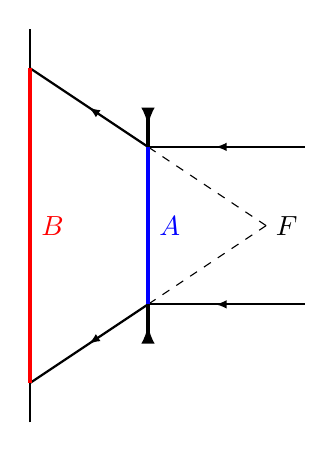
\begin{tikzpicture}[>=latex,scale=1.0]
  \draw[>-<, very thick ] (0,1.5)--(0,-1.5);
  \draw[thick] (0,1)--(2,1);
  \draw[thick] (0,-1)--(2,-1);
  \draw[>=latex, -<] (0,1)--(1,1);
  \draw[>=latex, -<]  (0,-1)--(1,-1);
  \draw[>=latex, ->] (0,1)--(-1.5/2,1.5);
  \draw[>=latex, ->]  (0,-1)--(-1.5/2,-1.5);
  \draw[dashed] (1.5,0)node[right]{$F$}--(0,1);
  \draw[dashed] (1.5,0)--(0,-1);
  \draw[thick] (0,1)--(-1.5,2);
  \draw[thick] (0,-1)--(-1.5,-2);
  \draw[thick] (-1.5,-2.5)--(-1.5,2.5);
  \draw [ultra thick, color=red] (-1.5,2)--node[right]{$B$}(-1.5,-2);
  \draw [ultra thick, color=blue] (0,1)--node[right]{$A$}(0,-1);
\end{tikzpicture}
\end{document}